%***************** FIELD THEORY ***************
\begin{frame}
	\begin{block}{Spaces and Coordinates}
		We compactify on:
		\begin{align*}
			\M_D                      & \to \M_{D-1} \times S^1    \\
			\eta_{\hat{\mu}\hat{\nu}} & = \text{diag}(-,+,\dots,+)
		\end{align*}
		With coordinates:
		\begin{align*}
			x^{\hat{\mu}} & = (x^\mu, y)      \\
			y             & \simeq y + 2\pi R
		\end{align*}
	\end{block}
	\begin{block}{Limits}
		\begin{equation*}
			E \ll \frac{1}{R} \ll \frac{R}{\alpha'}
		\end{equation*}
	\end{block}
\end{frame}

%********** SCALAR FIELD *********************
\begin{frame}{Scalar Field on \texorpdfstring{$S^1$}{S1}}
	\begin{block}{\texorpdfstring{$D$}{D}-Dimensional Real Scalar Field}
		The action is
		\begin{equation*}
			S_{D} = \frac{\Lambda^{D-4}}{2} \int_{\M_{d} \times S^1} \ud^D x \,  \de_{\hat{\mu}} \phi(x^{\hat{\mu}}) \, \de^{\hat{\mu}} \phi(x^{\hat{\mu}})
		\end{equation*}
		The equations of motion are
		\begin{equation*}
			\de_{\hat{\mu}} \de^{\hat{\mu}}  \phi(x^{\hat{\mu}}) = 0.
		\end{equation*}
	\end{block}

	\begin{block}{Compactification on \texorpdfstring{$\M_{D-1} \times S^1$}{M(D-1)xS1}}
		\begin{equation*}
			\phi(x^{\hat{\mu}}) = \sum_{s \in \Z} e^{isy/R} \phi_s(x^\mu),
		\end{equation*}
		\begin{equation*}
			\left( \de_\mu \de^\mu - \frac{s^2}{R^2} \right) \phi_s(x^\mu) = 0, \quad \forall s \in \Z,
		\end{equation*}
	\end{block}

\end{frame}

\begin{frame}{Scalar Field on \texorpdfstring{$S^1$}{S1}: Results}
	\begin{columns}
		\column{.5\textwidth}
		\begin{block}{Kaluza-Klein Masses}
			\begin{equation*}
				m^2_s = M^2 + \frac{s^2}{R^2}
			\end{equation*}
		\end{block}
		\column{.5\textwidth}
		\begin{block}{Negligible for}
			\begin{equation*}
				E \ll \frac{1}{R}
			\end{equation*}
		\end{block}
	\end{columns}
\end{frame}

%*********** EINSTEIN GRAVITY **********************
\begin{frame}{Einstein Gravity on \texorpdfstring{$S^1$}{S1}}
	\begin{exampleblock}{Decomposition \texorpdfstring{$SO(1,D-1) \to SO(1,d-1)$, with $d = D-1$}{Representations}}
		\begin{table}[c]
			\scalebox{0.96}{
				\begin{tabular}{|c|c|c|}
	\hline
	$SO(1,D-1)$                                          & $S=(1,d-1)$            & mode expansion                                                                              \\ \hline
	\multirow{3}{*}{$G_{\hat{\mu}\hat{\nu}} (x^\mu, y)$} & $G_{\mu\nu}(x^\mu, y)$ & $G^{(0)}_{{\mu} {\nu}} (x^\mu)+ \sum_{s \neq 0} G^{(s)}_{{\mu} {\nu}} (x^\mu) e^{is y / R}$ \\ \cline{2-3}
	                                                     & $G_{\mu d}(x^\mu, y)$  & $G^{(0)}_{{\mu} {d}} (x^\mu)+ \sum_{s \neq 0} G^{(s)}_{{\mu} {d}} (x^\mu) e^{is y / R}$     \\ \cline{2-3}
	                                                     & $G_{dd}(x^\mu, y)$     & $G^{(0)}_{{d} {d}} (x^\mu)+ \sum_{s \neq 0} G^{(s)}_{{d} {d}} (x^\mu) e^{is y / R}$         \\ \hline
\end{tabular}
			}
		\end{table}
	\end{exampleblock}
	\begin{block}{Zero Mode Ansatz}
		\begin{equation*}
			G^{(0)}_{\hat{\mu}\hat{\nu}} =
			\begin{pmatrix}
				e^{2\alpha_d} g_{\mu\nu} + e^{-2(d-2)\alpha_d \phi} A_\mu A_\nu & e^{-2(d-2)\alpha_d \phi} A_\mu \\
				e^{-2(d-2)\alpha_d \phi} A_\nu                                  & e^{-2(d-2)\alpha_d \phi}
			\end{pmatrix}
		\end{equation*}
	\end{block}
\end{frame}

\begin{frame}{Einstein Gravity on \texorpdfstring{$S^1$}{S1}}
	\begin{block}{Action and Decomposition for $D=5$}
		\begin{equation*}
			S_5 = \frac{M^3_5}{2} \int \ud^5 x \sqrt{-G} R_5
		\end{equation*}
		\begin{equation*}
			\ud s^2 =  e^{2\alpha_d \phi} g_{\mu\nu} \ud x^\mu \ud x^\nu + e^{-2(d-2)\alpha_d \phi} (\ud y + A_\mu \ud x^\mu)^2
		\end{equation*}
		\begin{equation*}
			S_4 = M^3_5 \pi R \int \udq x \sqrt{-g} \left( R_4 -\frac{1}{6} \de_\mu \phi \de^\mu \phi - \frac{1}{4 e^\phi} F_{\mu\nu} F^{\mu\nu} + \dots \right)
		\end{equation*}
	\end{block}

	\begin{block}{Results}
		\begin{equation*}
			M^2_p = 16 \pi^2 M^3_5 R,
		\end{equation*}
		\begin{equation*}
			\textup{Vol} (S^1)  = \int_{0}^{2\pi R} \ud y \, \sqrt{G^{(0)}_{yy}} = e^{-(d-2)\alpha_d \phi} \cdot 2\pi R .
		\end{equation*}
	\end{block}
\end{frame}

\begin{frame}{Brane-World Scenario}
	\begin{figure}[!h]
		\centering
		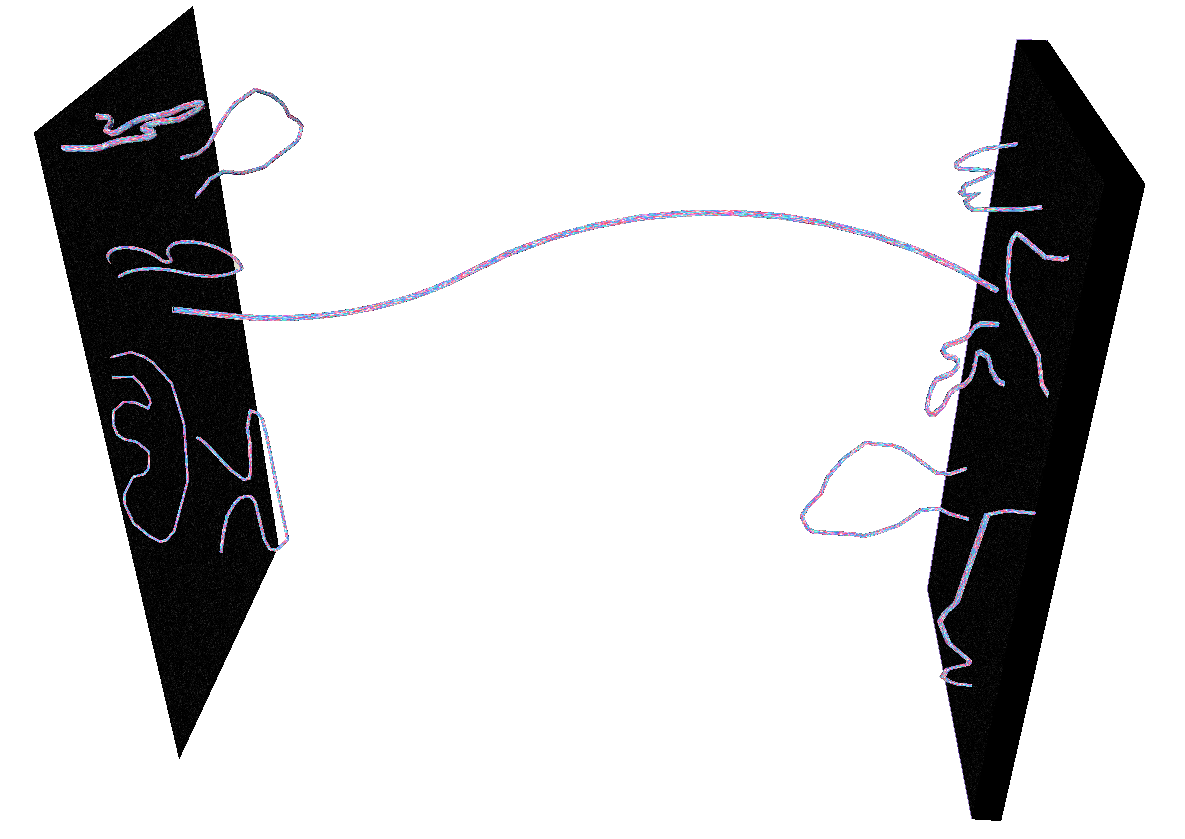
\includegraphics[width=50mm]{graphics/brane-world.PNG}
		\caption{Open strings attached to branes}
	\end{figure}
	\begin{block}{\texorpdfstring{We could have \texorpdfstring{$M_5\sim \text{TeV}$}{energy}, since $M^2_p = 16 \pi^2 M^3_5 R$}{Previous Relation}}
		\begin{equation*}
			S_\text{brane-world} = S_\text{brane} + S_\text{bulk} = \int \udq x \, \L_\text{brane} + \int d^{10} x \, \L_\text{bulk} .
		\end{equation*}
	\end{block}
\end{frame}

%************ BOSONIC STRING **************
\begin{frame}{Bosonic String: Lightcone Quantization}
	\begin{block}{The Setting}
		\begin{itemize}
			\item We work in $\M_{26}$, with \emph{closed strings} of length $l$;
			\item $\xi^a = (\tau,\sigma)$ on worldsheet. We use $\xi^\pm = \tau \pm \sigma$;
			\item We use $X^{{\mu}} \to (X^\pm, X^{{i}})$, with $X^\pm = {1}/{\sqrt{2}}(X^0 \pm X^1)$;
			\item $X^\pm$ can be fixed. The relevant ones are $X^i$, with \alert{boundary condition}
			      \begin{equation*}
				      X^i(\tau,\sigma+l) = X^i(\tau,\sigma)
			      \end{equation*}
			      for which
			      \setlength\abovedisplayskip{5pt}
			      \begin{equation*}
				      X^i (\tau,\sigma) = X^i_L (\xi^+) + X^i_R (\xi^-)
			      \end{equation*}
		\end{itemize}
	\end{block}
\end{frame}

\begin{frame}{Bosonic String: Lightcone Quantization}
	\begin{block}{Mode Decomposition}
		\setlength\abovedisplayskip{0pt}
		\begin{align*}
			X^i_L(\xi^+) & = \frac{x^i}{2} + \frac{\alpha'\pi}{l} p^i \xi^+ + i \sqrt{\frac{\alpha'}{2}} \sum_{n\neq 0} \frac{\tilde{\alpha}^i_n}{n}e^{-\frac{2\pi i}{l}n \xi^+}, \\
			X^i_R(\xi^-) & = \frac{x^i}{2} + \frac{\alpha'\pi}{l} p^i \xi^- + i \sqrt{\frac{\alpha'}{2}} \sum_{n\neq 0} \frac{{\alpha}^i_n}{n}e^{-\frac{2\pi i}{l}n \xi^-} .
		\end{align*}
	\end{block}
	\begin{block}{Level Matching and Mass-Shell}
		\setlength\abovedisplayskip{0pt}
		\begin{gather*}
			\tilde{N}_\perp =  N_\perp, \quad M^2 = \frac{2}{\alpha'} (\tilde{N}_\perp + N_\perp - 2) . \\
			\quad \tilde{N}_\perp \equiv \sum_{i=2}^{25}\sum_{n>0} \tilde{\alpha}^i_{-n} \tilde{\alpha}^i_n, \quad {N}_\perp \equiv \sum_{i=2}^{25}\sum_{n>0} {\alpha}^i_{-n} {\alpha}^i_n ,
		\end{gather*}
	\end{block}
\end{frame}

\begin{frame}{Bosonic String: Compactification on \texorpdfstring{$S^1$}{S1}}
	\begin{columns}[t]
		\column{.55\textwidth}
		\begin{block}{Compactification space}
			\setlength\abovedisplayskip{0pt}
			\begin{gather*}
				\M_{26} \to \M_{25} \times S^1 \\
				X^{\hat{\mu}} = (X^\mu, X^{25}), \quad y \simeq y + 2\pi R
			\end{gather*}
		\end{block}
		\column{.55\textwidth}
		\begin{block}{Lightcone coordinates}
			\setlength\abovedisplayskip{0pt}
			\begin{gather*}
				X^\pm = {1}/{\sqrt{2}}(X^0 \pm X^1) \\
				X^{\hat{\mu}} \to (X^\pm, X^{\hat{i}}) = (X^\pm, X^{i}, X^{25})
			\end{gather*}
		\end{block}
	\end{columns}
	\begin{block}{Boh}
		The \alert{local dynamics} is the \alert{same}. The global difference is
		\begin{gather*}
			X^{25} \simeq X^{25} + 2 \pi R \\
			X^{25}(\tau, \sigma + l) = X^{25}(\tau,\sigma) + 2 \pi R \omega, \quad \omega \in \Z
		\end{gather*}
	\end{block}
\end{frame}

\begin{frame}{Bosonic String: Compactification on \texorpdfstring{$S^1$}{S1}}
	\begin{block}{Mode Decomposition}
		\setlength\abovedisplayskip{0pt}
		\begin{align*}
			X^{25}_L(\xi^+) & = \frac{x^{25}}{2} + \frac{\alpha' \pi}{l} p_{\!_L} \xi^+ + i \sqrt{\frac{\alpha'}{2}} \sum_{n\neq 0} \frac{\tilde{\alpha}^{25}_n}{n}e^{-\frac{2\pi i}{l}n \xi^+} \\
			X^{25}_R(\xi^-) & = \frac{x^{25}}{2} + \frac{\alpha' \pi}{l} p_{\!_R} \xi^- + i \sqrt{\frac{\alpha'}{2}} \sum_{n\neq 0} \frac{{\alpha}^{25}_n}{n}e^{-\frac{2\pi i}{l}n \xi^-}.      \\
			\quad p_{\!_L}  & \equiv \left( \frac{s}{R} + \frac{\omega R}{\alpha'} \right), \quad p_{\!_R} \equiv \left( \frac{s}{R} - \frac{\omega R}{\alpha'} \right) ,
		\end{align*}
	\end{block}
	\begin{block}{Level Matching and Mass-Shell}
		\setlength\abovedisplayskip{0pt}
		\begin{gather*}
			\tilde{N}_\perp - N_\perp + s \omega = 0, \quad s,\omega \in \Z, \\
			M^2 = - p_\mu p^\mu = \frac{s^2}{R^2} + \frac{\omega^2 R^2}{\alpha'^2} + \frac{2}{\alpha'} (N_\perp + \tilde{N}_\perp - 2) .
		\end{gather*}
	\end{block}
\end{frame}


\begin{frame}{Bosonic String: T-duality}
	\begin{columns}
		\column{0.55\textwidth}
		\begin{block}{From Spectrum}
			\setlength\abovedisplayskip{0pt}
			\begin{align*}
				R & \to R' = \frac{\alpha'}{R}, \\ (s,\omega) &\to (s',\omega') = (\omega, s) ,
			\end{align*}
		\end{block}
		\column{0.55\textwidth}
		\begin{block}{From Full Theory}
			\setlength\abovedisplayskip{0pt}
			\begin{gather*}
				\quad p_{\!_L} \to p_{\!_L}, \quad p_{\!_R} \to - p_{\!_R} \\
				X^{25}_L \to X^{25}_L, \quad X^{25}_R \to -X^{25}_R
			\end{gather*}
		\end{block}
	\end{columns}
	\begin{block}{Boundary Condition}
		Let's see what happens under $\sigma \to \sigma +l$:
		\begin{align*}
			Y^{25}(\tau, \sigma) \to &Y^{25}(\tau, \sigma + l) = X^{25}_L (\xi^+ + l) - X^{25}_R(\xi^- - l) \\= &Y^{25}(\tau,\sigma) + \alpha' \pi (p_{\!_L} + p_{\!_R}) = Y^{25}(\tau,\sigma) + \frac{2\pi\alpha' s}{R} \\ = &Y^{25}(\tau,\sigma) + 2\pi R' s ,
		\end{align*}
		One can prove that the two \alert{theories} are the \alert{same}.
	\end{block}
\end{frame}

%********** SUPERSTRING *****************
\begin{frame}{Superstring: the Gluing}
	\begin{table}[c]
		\scalebox{0.79}{
			\begin{tabular}{|c|c|c|c|c|c|}
    \hline    sector & state rep. & $\alpha' M^2$ & statistics & $SO(8)$ (indices) & $SO(8)$ (dim.)  \\ \hline
        (NS$_-$,NS$_-$) & $\i \otimes \i$ & $-2$ & boson & / & / \\ \hline
        (NS$_+$,NS$_+$) &$\v \otimes \v$&$0$& boson& $[\boldsymbol{0}] \oplus [\boldsymbol{2}] \oplus (\boldsymbol{2})$ &$\boldsymbol{1} \oplus \boldsymbol{28_v} \oplus \boldsymbol{35_v}$\\ \hline
        (R$_+$,R$_+$) &$\s\otimes \s$&$0$& boson & $[\boldsymbol{0}] \oplus [\boldsymbol{2}] \oplus [\boldsymbol{4}]_+$ & $\boldsymbol{1_s} \oplus \boldsymbol{28_s} \oplus \boldsymbol{35_s}$ \\ \hline
        (R$_-$,R$_-$) &$\c \otimes \c$&$0$& boson & $[\boldsymbol{0}] \oplus [\boldsymbol{2}] \oplus [\boldsymbol{4}]_-$ & $\boldsymbol{1_c} \oplus \boldsymbol{28_c} \oplus \boldsymbol{35_c}$\\ \hline
        (R$_-$,R$_+$) &$\c \otimes \s$&$0$& boson & $[\boldsymbol{1}] \oplus [\boldsymbol{3}]$ & $\boldsymbol{8_v} \oplus \boldsymbol{56_v}$\\ \hline
        (R$_+$,R$_-$) &$\s \otimes \c$&$0$& boson& $[\boldsymbol{1}] \oplus [\boldsymbol{3}]$& $\boldsymbol{8_v} \oplus \boldsymbol{56_v}$\\ \hline
        (R$_+$,NS$_+$) &$\s \otimes \v$&$0$& fermion & / & $\c \oplus \boldsymbol{56_s}$\\ \hline
        (R$_-$,NS$_+$) &$\c \otimes \v$&$0$& fermion & / & $\s \oplus \boldsymbol{56_c}$\\ \hline
        (NS$_+$,R$_+$) &$\v\otimes\s$&$0$& fermion & / & $\c \oplus \boldsymbol{56_s}$\\ \hline
        (NS$_+$,R$_-$) &$\v\otimes\c$&$0$& fermion & / & $\s \oplus \boldsymbol{56_c}$ \\ \hline
    \end{tabular}
		}
	\end{table}
\end{frame}